\documentclass[12pt,MEng]{UoAThesis}
\usepackage{pdfpages}
\usepackage{biblatex}
\usepackage{float}
\usepackage{MnSymbol}
\usepackage{blindtext}
\usepackage{siunitx}
\addbibresource{ref.bib}

\makeatletter
\newcommand{\unchapter}[1]{%
  \begingroup
  \let\@makechapterhead\@gobble % make \@makechapterhead do nothing
  \chapter{#1}
  \endgroup
}

\thesistitle{\textbf{Winter Progress Report} \\Superconducting and Superinsulating Nanofluids}
\thesisauthor{Asad Mohiuddin}
\thesispdfkeywords{Nanofluid, Transient Heated wire, Thermal conductivity}
\thesisyear{2019}
\degree{MEng~degree in Chemical Engineering}
\thesisabstract{This projects aims to shed light on new physics that explores transient molecular effects in heat transfer of nanofluids. Through abstract molecular dynamics simulation of hard spheres performed by Dr Marcus Bannerman (supervisor) concluded that there is a short instant in time where they conduct a relatively large amounts of heat. This report will attempt to underline any relevant background of nanofluids that show why their thermal enhancement behaviour might be regarded as anomalous through classical models of heat transfer. More importantly an experimental approach is undertaken to determine if this anomalous behaviour can be measured through a comparatively inexpensive DIY design of the Transient Hot Wire technique. Design and experimental procedures have also been provided as a means to understand the direction of the project but these remain a work in progress and will continually be revised based on any new information as the spring term commences.}

\acknowledgements{Firstly I would like to thank a close friend and laboratory partner Niall McDonald for his support and company in the lab throughout summer and winter. His invaluable assistance and friendly personality has kept me highly motivated as well as developed my technical knowledge to undertake this project.

I would also like to thank PhD student Craig Moir for his collaboration as I look forward to working with him over the spring term.

Last but not least I would like to pay a very special thankfulness, warmth and appreciation to my supervisor and dear friend Dr Marcus Bannerman who has single handedly made this project possible. His support and patience with me at every point, his passion for science, and his generosity for funding this project (going way beyond the allocated budget for undergraduate projects), all of this, for which I am very much grateful for.
}


\begin{document}

\chapter{Introduction}
Heat transfer plays a vital role in a variety of different applications. For example, in automotives heat transfer affects the performance, emissions and durability of the engine including the design, and fatigue life of their respective components. Similarly the same applies to modern electronic that utilizes heat transfer for effective thermal management. Moore's Law is a well-known phenomenon that states that in highly dense integrated circuits (IC) the total number of transistors will approximately double every two years. Thermal management becomes unrealistic as the density of transistors with in the IC increase, thus a new challenge has appeared in heat transfer: cooling of nano-scale devices. A more efficient and compact design of heat exchangers is required for advanced nanoelectronics, and one way this can be achieved is through nanofluid technology. A very large enhancement of the thermal conductivity of a base fluid (i.e. water) can be achieved by the addition of highly conductive solid material in the form of nanoparticles. 

The mechanics of this enhancement have generally fallen into the classical/continuum bounds given by series and parallel resistances. These bounds are defined by two separate phases of the solid nanoparticles and the liquid medium and the arrangement of the nanoparticles with in the medium. If the nanofluid falls into these two limits then it can be said that these results are not anomalous, because they can simply be explained by the arrangement of the nanoparticles. But recently it has been demonstrated by Dr Marcus Bannerman and his fellow PhD student Craig Moir that anomalous thermal conductivity do exist in certain conditions, as a small number of these result do not fall into these bounds. Such as helium and hydrogen gas mixtures or the theoretical hard sphere model, which instead exhibit conductivity enhancements above the parallel bounds and dehancement below the series bounds, to an extent that it goes beyond the pure fluid values. These results have been predicted through equilibrium and non-equilibrium molecular dynamics, in compliance with Enskog Theory. These anomalous results can be explained by the movement of the species  in response to a temperature gradient. This behaviour is formally known as either thermophoresis, Soret effect or thermal diffusion. 

This query will be addressed and characterized through the use of theoretical, computational and experimental data. Specifically, this project will fixate on the on a construction of a Transient Hot Wire apparatus for testing the thermal conductivities of gas and liquid mixtures, which have similar dimensional properties to those of nanofluid systems, and use this experimental data to explore any anomalous heat transfer that may arise with in these mixtures.
 

\chapter{Nanofluids}
Modernised nanotechnology now provides the ability to engineer on a molecular and atomic scale to yield nanosized particles (or nanostructured polymers) that can have atleast one of their principle dimensions bellow 100nm. These additives can be present as types of oxide ceramics (e.g. Al$_{2}$O$_{3}$, CuO) or metal oxides (e.g. alumina, silica), also they can be a chemically stable metals, carbon in various forms or even metal carbides \cite{sheikholeslami2017applications}. In general, it is found that dilute multicomponent fluids of nanofluids have been used for the purpose of enhanced thermal performance. This is because the nanosized particles dramatically increase the thermal conductivity of the mixture compared to the pure fluid. The magnitude of this enhancement depend on the volume fraction, shape, size and arrangement of the suspended nanoparticles as well as their respective thermophysical properties. In fact, dilute concentrations of nanoparticles with as low as 1-5\% vol fractions, have demonstrated a thermal conductivity increase of around 60\% \cite{xuan2000conceptions, kakacc2009review}. In every physical mechanism the properties of a given materiel can change completely as it falls bellow a critical scale, this is where nanofluids exhibit enhanced thermophysical properties compared to their respective bulk forms. 

Nanofluids present unique features that have more advantages than from those of the conventional solid + liquid mixtures, in which the solid additive particles have physical dimensions that range from micrometer to millimetres. These mixtures tend to incorporate varity of issues such as eroded pipelines, clogged fluid flow, settling of solid particles and intense pressure drops \cite{xuan2000conceptions}. 

Current research on heat conduction of nanofluids consist of thermal conductivity measurements, extensions to existing models and development of new models for thermal conductivity predictions \cite{nanoreview}. However, there are still disagreements between the experiments and theories. 

\section{Mechanisms of Heat Conduction in Nanofluids}
Classical theories describe thermal conduction models by the arrangement of static nanoparticals suspended within a base fluid.

\begin{figure}[htp]
  \centering
  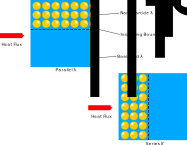
\includegraphics[clip,width=0.8\linewidth]{figures/seriesparralel}
  \caption{\label{fig:sp} Figure shows two-dimensional representation of the series and parallel model of thermal conduction in a binary nanofluid. Where the nanopartical is the dispersed within the base fluid. }
\end{figure}

The simplest model correspond to the series and parallel modes of thermal conduction. The conducting paths constitutes of a series or a parallel arrangement of the nonoparticles in the base fluid, with a perfectly insulating boundary present at the interface of the binary nanofluid. The effective thermal conductivities are given by:

\begin{equation}
 \frac{1}{\lambda^{\upvdash}}
 = \frac{1-\phi_p}{\lambda_f} + \frac{\phi_p}{\lambda_p}
\end{equation}

\begin{equation}
\lambda^{||} = ( 1-\phi_p ) \lambda_f + \phi_p \lambda_p
\end{equation}

\noindent Where $\lambda^{\upvdash}$ and $\lambda^{||}$ are the series and parallel limits of thermal conductivity, respectively. $\phi_p$ is the volume fraction of the dispersed nanopartical and $\lambda_p$ , $\lambda_f$ are the nanoparticle and base fluid thermal conductivities, respectively.Parallel defines the absolute upper limits of thermal conductivity as this is physically the best way of arranging nanoparticles because it provides a complete short-cut for heat to transferred, bypassing all the resistance of the base fluid. Whereas series defines the absolute lower limit of thermal conductivity as this is the worst way to arrange the nanoparticles. If the nanofluid's effective thermal conductivities go beyond the confinement of these limits they are regarded as anomalous, as it does not make sense considering simple heat transfer. 

The series and parallel limits are not the narrowest limits that can estimate the thermal conductivities in nanofluids using the classical approach. Maxwell theory also contains an upper and lower limit. Maxwell considered a heterogeneous medium that contains dilute suspension of spherical nanoparticles for which they are far enough apart from one another, that their interactions can be neglected. Looking far away enough from the nanoparticles that they are collected near the origin, then consider a sphere around the origin of the nanoparticles whose radius is such that it fits the correct packing fraction. The effective thermal conductivity of this larger sphere gives the same thermal conductivity of having all the individual dispersed nanoparticles.


\begin{figure}[htp]
  \centering
  
\includegraphics[clip,width=0.6\linewidth]{figures/maxwell}
  \caption{\label{fig:maxwell} Figure illustrates the strategy behind Maxwells theoretical model of dispersed particles within a heterogeneous system such that the base fluid is the continuous phase.}
\end{figure}

\noindent The upper limit of Maxwell theory constitutes the configuration in which the nanoparticles are in the dispersed phase and the base fluid in the continuous phase. Upper limit is given by \cite{class2010}:

\begin{equation}
\lambda^{\uparrow}_{eff} = \lambda_p \left( 1 - \frac{3(1 - \phi)(\lambda_p - \lambda_f)}{3 \lambda_p - \phi(\lambda_p - \lambda_f)} \right)
\end{equation}

\noindent Whereas the lower limit of Maxwell theory, the base fluid is in the dispersed phase and the nanoparticles are in the continuous phase. Lower limit is given by \cite{class2010}:

\begin{equation}
\lambda^{\downarrow}_{eff} = \lambda_f \left( 1 + \frac{3 \phi (\lambda_p - \lambda_f)}{3 \lambda_f + (1 - \phi)(\lambda_p - \lambda_f)} \right)
\end{equation}

\noindent Where $\lambda^{\uparrow}_{eff}$ and $\lambda^{\downarrow}_{eff}$ are the upper and lower limit effective thermal conductivities respectively and $\phi$ is the volume fraction of the dispersed phase.  

\begin{figure}[htp]
  \centering
  \includegraphics[clip,width=0.62\linewidth]{figures/limits}
  \caption{\label{fig:maxwell} Comparison of Maxwell limits to series and parallel. Here $\lambda_p = 10$ and $\lambda_f = 1$. }
\end{figure}

\noindent There are extensions to Maxwell theory that accompanies new parameters such as the shape of the nanopartical, or a film resistance on the nanopartcle instead of a no-slip condition. The magnitude of these parameters are unknown and practically impossible to determine. 

\begin{figure}[htp]
  \centering
  \includegraphics[clip,width=1\linewidth]{figures/ana}
  \caption{\label{fig:ana} Figure of Ref. \cite{class2010}: Each figure show classical bounds for thermal conductivity in specific nanofluids. The thin solid and thin dashed-dotted lines denote enhancement of thermal conductivity with in series and parallel limits. The upper Maxwell limit is denoted as the thick black line while the lower Maxwell limit is the dashed line. The markers show experimental data.}
\end{figure}

Figure \ref{fig:ana} shows the classical bounds along with experimental data of nanofluids, where water is the base fluid with solid additives of specific nanoparticles. It can be seen that at certain volume fraction Water-Fe$_3$O$_4$ can have enhancements above the parallel limit. Water-Fullerene (also known as Buckminsterfullerene with the chemical formula C$_{60}$) shows enormous dehancements bellow the series limit. These nanofluids are said to show anomalous behaviour in thermal conduction, as classical conduction fails to predict them.

\section{Thermophoresis}
This project assumes that anomalous heat transfer of nanofluid systems can be explained by the affect of thermophoresis. Thermophoresis is a very complicated transport effect and there is yet to exist a precise practical description explaining the intuition behind it, despite more than 150 years of research since Ludwig and Soret. When a temperature gradient $\nabla T$ is applied across a binary heterogeneous system there will be a resulting mass flux of both species, where the fluid does not flow. This mass flux of a single species  $J_m$ is given by \cite{sovet2004}:

\begin{equation}
J_m = - \rho D \nabla C - \rho C (1 - C) D_T \nabla T
\end{equation} 

\noindent Where $\rho$ is the density, $C$ is the particle concentration (in mass fraction), $D$ is the diffusion coefficient from Ficks law and $D_T$ is the thermal diffusion coefficient of one species. For gaseous mixtures, thermophoresis can be predicted using Chapman-Enskog theory. While there is currently no theoretical model that predicts this affect for liquid mixtures \cite{sovet2004}.

Figure \ref{fig:thermo} shows the effect of thermophoresis. Due to the temperature gradient the bigger particles (Species B) gain a drift velocity that brings them closer to the hot wall, while the smaller particles (Species A) obtain an opposing drift velocity that moves them closer to the colder wall, this is known as positive thermophoresis. With negative thermophoresis the bigger particles move towards the cold wall, and smaller ones to the hot wall.

\begin{figure}[htp]
  \centering
  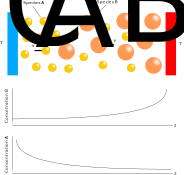
\includegraphics[clip,width=1\linewidth]{figures/thermo}
  \caption{\label{fig:thermo} Figure illustrates the effect of thermophoresis on particle distribution on a binary heterogeneous system.}
\end{figure}

\chapter{Transient Hot Wire}
The transient hot wire (THW) is a well established non-steady state technique to determine the effective thermal conductivity of gasses, liquids, nanofluids and even solids. It is favoured over other techniques primarily due to short test times and accuracy. The heart of this technique involves an extremely thin metallic wire that is completely submerged into the sampling materiel and serves 2 critical roles. The wires first role is to act as a heat source; this is exploited through the Joule's effect. When a potential difference $ V $ is placed across the length of the wire $l$; electrons will flow through it, this is known as current $I$. As the electrons travel through the wire all of their potential energy is converted into thermal energy (Joule's heat) by collisions with the crystal lattice of the metallic wire. 

\begin{equation}\label{eq:heat1}
q = \frac{I V}{l}
\end{equation}

\noindent Where $q$ is the amount of Joule's heat generated per unit length by of the wire that is spread radially into surrounding medium.

\begin{figure}[htp]
  \centering
  \includegraphics[clip,width=0.4\linewidth]{figures/basicTHW.pdf}
  \caption{\label{fig:testfig} Cross sectional view of the hot wire, displaying heat release from the wire as a result of Joule's effect.}
\end{figure}

\noindent The second role of the wire is to serve as a temperature sensor. The temperature of the wire is found through empirical relationships of the metal wires electrical resistivity and its temperature. Typically these types of relationships are determined through \emph{in situ} calibration of the metallic wire. 

Assuming that the wire is initially equilibrium, at time $t = 0$ a step change in voltage is applied across the wire. The evolution of the temperature of the wire with time is determined by the thermal conductivity of the medium surrounding it. It is important to note that this method is labelled as transient because the power is applied quickly and the measurements are taken over a short period. 

Ideally, there is a linear heat source that is infinity and infinitely thin to an infinite incompressible homogeneous medium, where the temperature of the hot wire varies with time. Relative to the medium, the heat generated by the hot wire is treated as a boundary condition. Then the basic problem that is driven by the non-stationary heat diffusion of Fourier's law becomes:

\begin{equation}
\frac{\partial T}{\partial t} = \alpha \nabla^2T
\end{equation}

\noindent Where $\alpha = \frac{\lambda}{\rho C_p}$ the thermal diffusivity of the medium, the ability of the medium to conduct thermal energy relative to its ability to store it. The density $\rho$ of the medium is approximated through an equation of state from experimentally measured temperature and pressure. The heat capacity of the medium as $C_p$ and its thermal conductivity as $\lambda$. 

With the appropriate boundary conditions the solution to this problem is well known and analytically proven by Carslaw H S and Jaeger J C in 1959 \cite{carslaw1959}. The solution at a spacial domain $r$, along with the complete integral expansion is found to be:

\begin{equation}
\Delta T_{ideal}(r,t) = \frac{q}{4 \pi \lambda} \left[ \ln \left( \frac{4 \alpha t}{r^2 C}\right) + \frac{\left( \frac{r^2}{4 \alpha t} \right)}{1(1!)} + \frac{\left( \frac{r^2}{4 \alpha t} \right)}{2(2!)} + ... \right]
\end{equation}

\noindent Where $ C = e^{\gamma} = 1.781 $ is the exponential of Euler's constant. In most application it is sufficient to just take the first term of the integral expansion as $r$ is small and $\alpha t$ is comparatively large. Also that the surface of the hot wire imposes a uniform temperature which is equal to that in the conducting medium at $r = r_0$. The ideal equation describing the temperature history of the wire then becomes:

\begin{equation} \label{eq:ideal}
\Delta T_{ideal}(r_0,t) =  \frac{q}{4 \pi \lambda} \ln \left( \frac{4 \alpha t}{r^2_0 C}\right)
\end{equation}

\noindent Therefore at a fixed radial distance the thermal conductivity is defined as:

\begin{equation} \label{eq:straight}
\lambda =  \frac{q}{4 \pi} \frac{d\ln \left( t \right)}{d\Delta T_{ideal}}
\end{equation}

\noindent From Eq. \ref{eq:straight} the typical ideal plot for the temperature change of the wire against the logarithmic time, for an ideal experiment of the THW will propose a straight line. 


\section{Relevant Design Background}
Thermal conductivity measurement have been divided into two distinctive groups, steady state and non-steady state methods. To explore transient effects in the thermal conductivity of colloidal systems, the non-steady state technique is to be adapted. Consideration on recent non-steady state techniques such as: transient plane source \cite{tps}, 3-omega \cite{omega} and the thermal constants analyser \cite{tca} concluded that the construction of these devices are complicated and have potential for high costs. Where as the popular transient hot wire technique (THW) is more favourable due to its simplicity in design and construction. After the work of Healy et al \ref{thoery} it is found that the THW technique can predict the thermal conductivity of gases with a percision of 0.02\% and an accuracy of of 0.2\% with temperatures and pressures up to \SI{800}{\celsius} and \SI{400}{atm}.

To achieve an accurate assessment of thermal conductivity of a fluid the technique must be able to isolate effects of convection and radiation. The contribution of convection becomes apparent when the graph of $\Delta T$ as a function of $ln(t)$ departs from linearity. If the measurement time is short-lived there will not be enough time to generate convective currents in the sampling fluid \cite{groot}. When determining the thermal conductivity, corrections are available on literature to account for divinations from the ideal state (e.g. radiative heat transfer, Knudsen effect etc.). These corrections, $\delta T_i$, are applied to the measured temperature changed of the wire.


\begin{figure}[htp]
  \centering
  \includegraphics[clip,width=1\linewidth]{figures/newTHW}
  \caption{\label{fig:newthw} Figure of Ref. \cite{history}: Modern variations of the transient hot wire apparatus.}
\end{figure}

By the 20th century the hot wire technique became very common, especially after the solution to the ideal analytical model and the advances in electronics (i.e. more accurate and faster digital multi meters) thus giving rise to the more profound ``transient'' hot wire technique. Figure \ref{fig:newthw} shows modern designs incorporating new tricks to improve the accuracy and reliability of measurements for any given fluid. 

All the designs in Figure \ref{fig:newthw} encompasses two hot wires of dissimilar lengths, where the shorter wire is used to cancel out any end effects. It should also be mentioned that the cells and hot wires are designed to be placed vertically so that the Earth's gravity is perpendicular to the temperature gradient imposed by the hot wires, thus reducing the occourance of natural convection. Design (a) utilizes extremely thin Platinum wire with a diameter of \SI{7}{\micro\meter} that are fixed on both ends. Wires at this diameter are Wollaston processed, this means that the Platinum wire initially contains silver cladding. Once the wire is fitted in place, it is transferred to an acid bath to dissolve the silver cladding. These types of wire are typically impractical to handle and are also too fragile. Design (b) is similar but more rational, the Platinum wire is not Wollaston processed but instead is \SI{10}{\micro\meter} in diameter, furthermore springs are in place keep the wire taunt. Design (c) replaced the spring for a weight to account for thermal expansion when the wire is heated. This design also swapped out Platinum for Tantalum, to allow the  measurement of thermal conductivity on electrically conducting liquids. Oxidation of Tantalum forms an electrically insulating layer of Tantalum Pentoxide, but a correction must be applied when computing the thermal conductivity \cite{elec}. Design (d) and (e) discarded the weight, but instead employs a wire support made out of Tantalum, allowing them both to thermally expand simutaneously to always keep the wires taunt \cite{history2}.
 

\section{Design \& Construction}
Platinum as the materiel for the hot wires is chosen specifically for its well known resistance temperature relationship and also its naturally high resistivity allowing for greater accuracy in resistance measurements. The wire should mimic the ideal line source model as much as possible. The wire diameter is \SI{15}{\micro\meter} as this minimizes the effects of its finite diameter additionally providing high resistance while retaining reasonable tensile strength for the present application.

\subsection{Wheatstone Bridge}

The principle concept of the THW technique is reasonably straightforward. The measurement to be performed is temperature rise by the determination of resistance variations, whilst providing a constant current. Resistance measurements are performed by providing known current and measuring the relative voltage drop across the resistive elements, the resistance is computed using Ohms law:

\begin{equation} \label{eq:ideal}
R = \frac{V}{I_S}
\end{equation}


Precise resistance measurements can be accomplished by either the 4 wire technique or by using a Wheatstone bridge.
The Wheatstone bridge, a classical technique that is commonly applied for temperature measurements, was selected for this design. The schematic can be seen in Figure \ref{fig:WB} with reference to Table \ref{Rtable}. The ideal line source model assumes that the wire is infinitely long so that heat is not conducted axially from both ends of  of the wires, so a 2 wire system is adapted to eliminate these end effects. This is achieved by placing the long hot wire on one working arm of the bridge, and the short hot wire on the other. Assuming that the bridge is initially balanced (i.e. $V_{AB} = 0 $), the voltage developed between nodes A and B will be the result of the resistance variations due to temperature rise of both the wires. End effect compensation comes from the ability for the Wheatstone bridge to automatically provide a direct subtraction of resistance changes of the hot wires. The resulting effect is that a finite length of the hot wire approximates that of a infinity long hot wire. Therefore, it is useful to talk in terms of the effective length $l_W = l_L - l_S$ and effective resistance $R_W = R_L - R_S$ of the hot wires.

For the bridge to be balanced the potentiometers have to be adjusted until this equality is satisfied:

\begin{equation} \label{eq:balance}
\frac{R_S + R_3}{R_L + R_1} = \frac{R_4}{R_2}
\end{equation}

\noindent The voltage profile that is developed across nodes A and B can be expressed as:

	\begin{equation} \label{eq:V_wb}
V_{AB}(t) = \left( \frac{R_1 + R_L(t)}{R_1 + R_L(t) + R_3} - \frac{R_4}{R_2 + R_S(t) + R_4} \right) V_S
	\end{equation}

From the voltage profile, Eq. \ref{eq:V_wb}, it is crucial that the resistances of the potentiometers do not vary during the measurement period. As discussed, variations in resistance arise from temperature changes, therefore the potentiometers selected should have a low temperature coefficient (low response to temperature changes). Voltage sense leads are placed closely across every resistive element to to obtain accurate individual resistances. 

\begin{figure}[h]
  \centering
  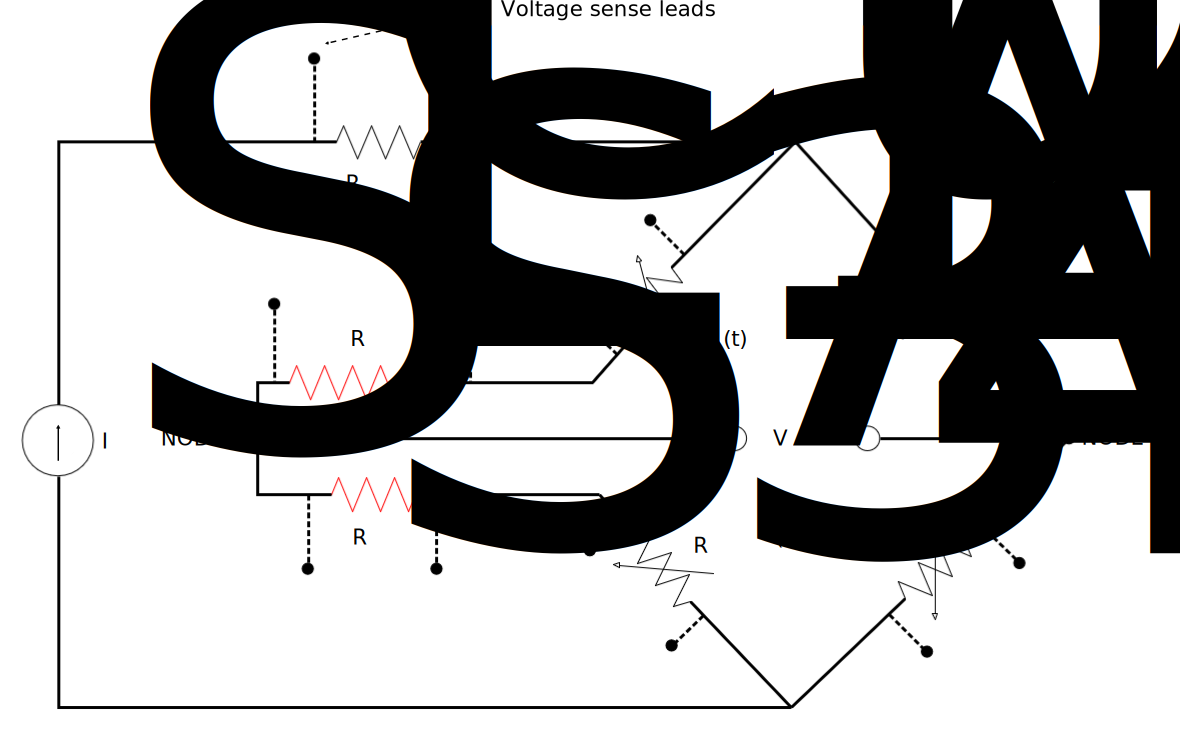
\includegraphics[clip,width=1\linewidth]{figures/WBcircuit.pdf}
  \caption{\label{fig:WB} Electrical schematic of the THW, that integrates a Wheatstone bridge with 2 wires of dissimilar lengths. In reference to Table \ref{Rtable}.}
\end{figure}

\begin{table}[htp]
\begin{center}
\begin{tabular}{ccccc}
\hline
Resistor                 & Component          & Resistance ($\Omega$) & Tolerance (\%) & \begin{tabular}[c]{@{}c@{}}Temperature \\ Coefficient (\SI{}{ppm\per\celsius})\end{tabular} \\ \hline
$R_{Current} $             & Precision Resistor & 100                 & $\pm 10$            & $\pm 100$ \\
$R_L$ at \SI{20}{\celsius} & Long Pt Wire      &  N/A                  & N/A           & $\pm 38.5$* \\
$R_S$ at \SI{20}{\celsius} & Short Pt Wire     &  37.72                   & N/A           & $\pm 38.5$* \\
$R_1 - R_4 $               & Potentiometers     & 0 - 200             & $\pm 10$           & $\pm 100$ \\ \hline
\end{tabular}
\end{center}
\caption{Resistive elements that are present on the THW circuitry, in reference to Figure \ref{fig:WB}. ( * ) are typical temperature coefficient values for pure platinum.}
\label{Rtable}
\end{table}

 A major challenge to achieve accurate resistance measurements is to nullify the loading effect of the circuit from the digital voltmeter (DVM). These inaccuracies arise since the DVM draws a small amount of power from the circuit, even though the DVM has a relatively high impedance (e.g \SI{50}{\mega\ohm}). Another advantage of using the Wheatstone bridge is; when the bridge is balanced the DVM does not draw any power from the circuit, hence increasing accuracy by nullifying the loading effect \cite{wb}. 

\subsection{Printed Circuit Board}

The THW proposed within this project did not follow the structural arrangements displayed in Figure \ref{fig:newthw}. Instead, the approach incorporated a printed circuit board (PCB) that includes the external circuitry along with both the wire supports and their electrical connections, also a milled out window for the cell around the Platinum wires. Figure \ref{fig:eagle} shows the finalized PCB design through a CAD software: EAGLE.

\begin{figure}[htp]
  \centering
  \includegraphics[clip,width=1\linewidth]{figures/eaglesch.pdf}
  \caption{\label{fig:eagle} EAGLE CAD board design showing specific layers that include copper traces, component pads/through-holes, drill holes, milling etc... The complete board size is \SI{200}{\milli\meter} by \SI{100}{\milli\meter} (not to scale).}
\end{figure}


This method of creating a THW system has its advantages and disadvantages over the coaxial methods presented in Figure \ref{fig:newthw}. Such benefits include: A more compact instrument, as external circuitry and hot wires are coexisting. Also that predefined lengths of hot wires are set with high accuracy. Lengths from the wire support via's are \SI{93.68}{\milli\meter} and \SI{64.69}{\milli\meter}, for the long and short hot wire respectively. Also, an inexpensive design as the price for printing 20 boards from overseas is around £60 (without parts). A drawback of this design is that the it ignores thermal expansion of the wire due to temperature changes, as there is no weight/spring to always keep the wires taunts. This is not too problematic as the thermal expansion coefficient of platinum is small, also temperature rise of the hot wire will be minimal for this application. 

The electrical connectivity and support of the wire is shown in Figure \ref{fig:wiresup} which displays part of a 3D drawing of the PCB. It is important that the hot wires are kept straight as they project across board. This is achieved by first resting both ends of the wire on top of the wire gap (in-between the SMD pads), next it is dragged through the wire via with slight force to keep the hot wire taunt and free of any kinks. It is important that the hot wire has no kinks as they can create axial heat conduction, deviating it from the ideal line source that of which the the shorter wire can not compensate for. The hot wire is then soldered on to the SMD pads so it is electrically connected to the copper traces on the 2nd layer (yellow fill shown in Figure \ref{fig:eagle}) inside the PCB by the via. To prevent the solder from connecting the hot wires to the top copper layer of the board the solder mask is left on the wire supports. 

\begin{figure}[htp]
  \centering
  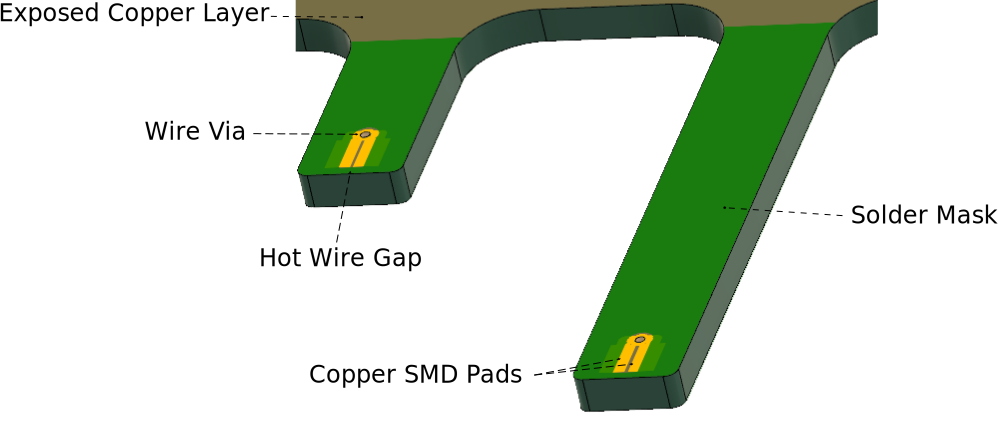
\includegraphics[clip,width=0.7\linewidth]{figures/wiresupport.pdf}
  \caption{\label{fig:wiresup} Fusion 360 drawing of the PCB showing the wire supports also highlighting the features of the wire connectivity.}
\end{figure}

The PCB is a 4 layer board where the first layer (top layer) and last layer (bottom layer) are almost completely covered by copper to act as shielding layers. This protects the board from electromagnetic interference (EMI) that is emitted by the surrounding environment, thus aiding to reduce digital noise when taking precise measurements. EMI shielding is achieved by running copper traces between the shielding layers. For every component SMD pads there is a corresponding via that connects to either the 2nd or 3rd layer, where the traces lie. These traces link the Wheatstone bridge and contain the voltage sense lines, they are depicted as the yellow and green fills on Figure \ref{fig:eagle}.

The traces are made of copper, but copper itself is not a perfect electrical conductor, it also has resistance. The expression \cite{pcb} relating to the resistance of a trace, $R$, is given by:

\begin{equation} \label{eq:Rtrace}
R = \rho \frac{L}{HW}\left[1 + \alpha \left( T - 25 \right) \right]
\end{equation}

\noindent Where H, L and W represent the physical dimensions of the trace, i.e. the height, length and width, respectively. T as the temperature of the trace in \SI{}{\celsius}. $\alpha$ represents the temperature coefficient and $\rho$ as the electrical resistivity of copper. For design optimization using Eq. \ref{eq:Rtrace}, to compensate for the PCB trace resistances can be accomplished by increasing the trace area for a given length of a trace. This is done for the traces that supply current across each component of the whetstone bridge, so that the magnitude of the resistances of the hot wires and potentiometers are far greater than those of the copper traces. Increasing the heights of the traces is another option but this greatly increases the total cost of the PCB. 

From Figure \ref{fig:eagle} it can be observed that the potentiometers on the Wheatstone bridge are compact. This is done intentionally to keep them at the same temperature so that any thermal response cancels out. In fact, thermal grease covering the potentiometers will ensure that they are well thermally coupled.

There are 6 1206-SMD pads around the milled out window for thermistors. All the thermistors are placed in series from a separate current supply. Voltage sense traces are also placed as close as possible to the thermistors, and like-wise with the hot wires, the resistance will be computed using ohms law to find the temperature of the cell. It is important that a small current is placed across the thermistors to keep heat dissipation to the cell a minimum. 

The power traces and voltage sense traces run to the top of the board to one of the 5 shielded Cat6 Female RJ45 connectors. These type of connectors are ideal for nullifying electrical noise as they very well shielded from electromagnetic interference and electrical cross-talk, external wiring is known to be the most susceptible to EMI and electrical cross-talk. These connectors gives the ability to use Ethernet cables, in particular Cat8 Ethernet cable shown in Figure \ref{fig:cat}.

 \begin{figure}[htp]
  \centering
  \includegraphics[clip,width=0.4\linewidth]{figures/cat}
  \caption{\label{fig:cat} Figure of Ref. \cite{cat8}: The Cat8 Ethernet cable used for externally wiring the PCB to a DMM or D/A. The figure highlights the features to ensure that the cable is well protected from EMI and electrical cross-talk.}
\end{figure}

\noindent When current flows through a wire a magnetic field will be imposed across the wire. Twisting the wires along their path reduces EMI and cross-talk as the magnetic field produced by one wire is cancelled by the magnetic field produced by the other, since they carry equal and opposite amounts of current. The drain wire is used in conjunction with the metallic shields to ensure effective grounding. The drain wire is in contact with the shield throughout the length of the wire. When the drain wire is grounded, any unwanted electrical noise will then be carried away from the circuit to ground.

\subsection{Cell Design and Fabrication}

The idea behind the cell design in shown is Figure \ref{fig:cell}. When assembled the cell provides two hollow cylindrical wells \SI{9}{\milli\meter} in diameter and \SI{10}{\centi\meter} in length, where the PCB rests in middle to accommodate both hot wires so they are suspendedalong the centeral axis of the capsulating cells to avoid the effects of the cell walls. To reduce the chances of natural thermal currents it is necessary to keep the cell diameter and wire lengths small \cite{groot}. Small cut out slots are also present on the cells to allow SMD thermistors to be fitted within the cells. Threaded holes are placed optionally on the cells parallel to the PCB holes, in-case the cells are required to be screwed together. One major design consideration is to keep both halves of the cells and PCB well thermally coupled. This is achieved by placing multiple extruded lips that pass through the PCB to the opposing cell. Also, the solder mask is peeled back, to expose the bare copper layers where the cell contacts the PCB. On top of that, numerous stitching via's are placed all over these contact areas to achieve greater coupling of the cells and PCB, this is more visible from Figure \ref{fig:eagle}. 

\begin{figure}[htp]
  \centering
  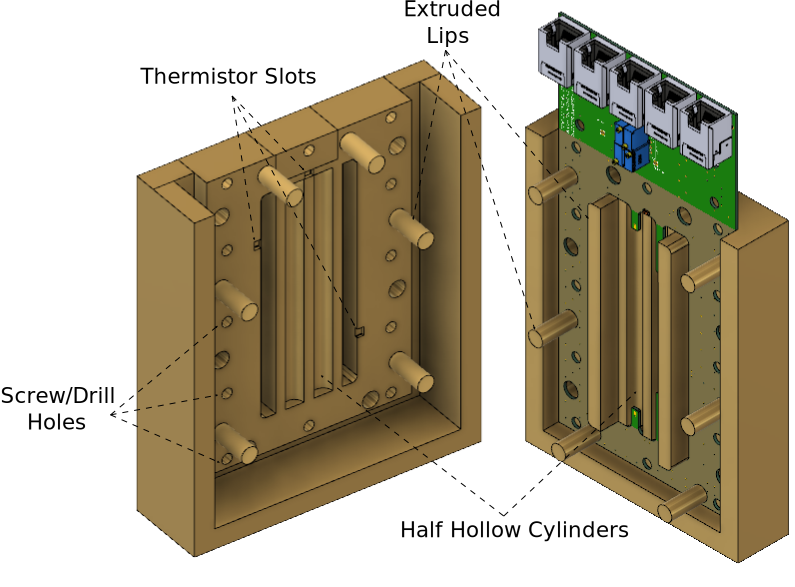
\includegraphics[clip,width=1\linewidth]{figures/cell}
  \caption{\label{fig:cell} Fusion 360 drawing of both halves of the cell and the PCB (not finalized cell design). When both cell halves adjoin a complete \SI{9}{\milli\meter} diameter cylinder is formed between the hot wires, where both hot wires will rest in the central axis}
\end{figure}

Two holes drilled into to each of the hot wire wells will provide a path for fluid to enter the vessel, by the means of a small capillary tube. A pressure sensor containing piezoresistive transducer will be fitted to check if the cell is at constant pressure. Valves will control the flow of liquid in and out the vessel.

\section{Experimental Procedures}

\subsection{Instrument Calibration}
Resistance temperature relationship of both platinum wires have to established through \emph{in situ} calibration. This requires the cell to be immersed in a liquid thermostat bath where temperature of the cell are to be taken from high precision thermistors on the PCB. But firstly the SMD thermistors should be confirmed on their accuracy by a secondary thermocouple. Resistance measurements of the hot wire are to be performed at different currents to find a suitable current that will give an accurate measurement of resistance without heating the wire itself. 

\begin{figure}[htp]
  \centering
  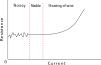
\includegraphics[clip,width=0.6\linewidth]{figures/cal.pdf}
  \caption{\label{fig:cal} Figure shows a prediction of recording the resistance of the hot wire at varying currents, using the four terminal method.}
\end{figure}

\noindent Resistance measurements are taken using the four terminal method at various temperatures from a selected current in the stable regime. The resulting data is then fitted to find the resistance relation for each wire by the following analytical function: 

\begin{equation} \label{eq:cal}
R(T) = A + BT + CT^2
\end{equation}

\noindent Where T is the temperature in Kelvin.

\subsection{Measurement Process}
VXI mainframe is adapted to provide both the tools and flexibility for operating the transient hot wire experiment. Introduced in 1987, VXI mainframe allows addition of diverse Eurocards (modules) providing trigger lines, a local bus, and other functions suited for a broad range of measurement applications. An Agilent E1406A Command Module translates SCPI (Standard Commands for Programmable
Instruments) for Agilent register based instruments through a General Purpose Interface Bus (GPIB). For the THW experiment specific Agilent modules are employed. Foremost 6.5 digital multimeters (DMM) for high accuracy voltage readings. In conjunction to a multiplexer module that switches up to 16 channels, where each channel provides High (H), Low (L), and Guard (G) connections. The HP E1328A 4-Channel D/A Converter, 16-bit isolated digital-to-analog channels that is configurable for providing an accurate current output. 

A potential scheme incorporating the VXI modules for the THW experiment is shown in Figure \ref{fig:VXI}. The voltage sense lines on the PCB are connected to the multiplex via multiple Ethernet cables. The multiplexer is connected externally to the High, Low Guard inputs of the DMM. Current for the Wheatstone bridge and thermistors are supplied through the D/A which is also connected by a single Ethernet cable. The timing and measurements are controlled by a micro-controller, that externally triggers the switching between the channel and measurement readings, also triggers the D/A through the command module. 

\begin{figure}[htp]
  \centering
  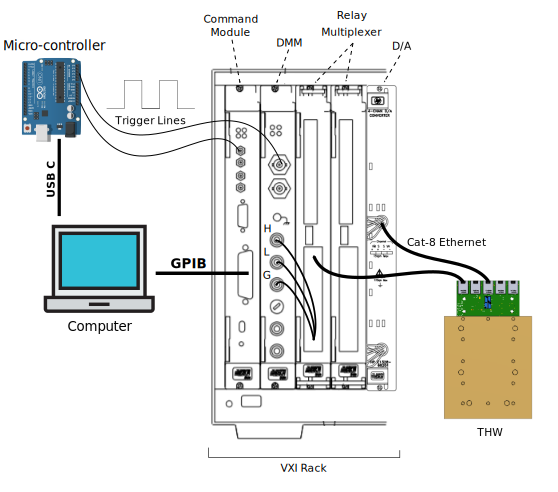
\includegraphics[clip,width=1\linewidth]{figures/VXI.pdf}
  \caption{\label{fig:VXI} A possible scheme to take THW readings using the Agilent/HP VXI mainframe from relevant modules.}
\end{figure}

\subsection{Description of Method}

The initial experiments will primarily focus on measuring the thermal conductivity of gasses, in particular hydrogen and helium. To begin with the gasses will both be tested separately, the results then compared to other sources to see how well the apparatus has performed. The sequence of events during an experiment follows 2 subsequent phases. 

The first phase involves balancing the Wheatstone bridge so that the voltage across the nodes of the bridge are as close to null as practical. A small current is used that creates negligible heating of the wire (stable zone in Figure \ref{fig:cal}) applied to the bridge to allow four wire resistance measurements to be taken place across all the resistive elements through the multiplexed DMM. The potentiometers are adjusted until the equality in Eq \ref{eq:balance} is satisfied, or more simply by making the total resistance in each four legs of the bridge the same. It is important that resistances are known very precisely in order to obtain accurate value of thermal conductivity of the sampling gas.

Second phase commences after achieving a satisfactory bridge balance.  The D/A is then set to drive a current that will produce desired heating of the hot wires. The experiment is then initiated by applying it across the bridge, during the experiment the DMM records the bridge voltage $V_{ab}$ as a function of time. This signal is proportional to the change in the effective resistance of the central section of the wire $R_w$. Consequently the temperature rise $\Delta T_w$ is determined from the current applied to the bridge, the measured bridge voltage and the two hot wire calibrations. During the experimental run the current applied to the bridge will change due the change effective resistance of the bridge. So if possible, voltage across $R_{current}$ should also be continually measured to find the exact power applied to the bridge at any given time. The ideal temperature rise is obtained after adding a number of corrections to the experimental temperature rise, to closely approximate the ideal line-source model.

\begin{equation} \label{eq:correction}
\Delta T_{ideal} = \Delta T_w + \sum_{i} \delta T_i
\end{equation}

\noindent The thermal conductivity is found by determining the slope of linear fit in the exponential rise in temperature $\Delta T_{ideal}$ as it reaches steady state. 

The next experiments will entail a binary mixture of the gas containing Hydrogen and Helium. It is expected that all of a sudden to due to thermophoresis that the thermal conductivity will be incompetent with in the binary gas. To measure and quantify the thermal conductivity coupled with thermophoresis, it will be ideal if the wires are cycled to put heat in and take heat out the sampling gas. This is impossible, so instead the power used to heat the wire will be sinusoidal as a function of time. It is expected that this will create an oscillation on the temperature profile of the wire $\Delta T$ vs $ln(t)$ plot. If the frequency is high the oscillation will be very small that it will mimic the typical exponential line. But what will be interesting to see is what happens when the frequency is decreased. It is believed that this data will show thermal conductivity coupled with the effects of thermophoresis, provided the diffusion rate of the species is small enough to be measured physically. Hydrogen-Helium mixture is found to exhibit positive thermophoresis, as the hot wire heats up large Helium particles move closer to the wire while the small Hydrogen particles move to the wall. As the wire gets colder (partially switched off) the opposite movement of the particles occurs. 





\chapter{Work Plan for Spring Term}

This chapter will briefly outline the main objectives, hoped to be accomplished throughout the spring term, as well as providing a Gantt chart to show their corresponding time-lines. 


\section{Transient Hot Wire}
Design and construction of the hot wire apparatus is still required to be completed before any thermal conductivity measurements of gasses can be taken place. First and foremost the cell design has to be finalized with the mechanical work shop so that milling of the cell can initiate, along with fittings for the cell so that compressed gas can be transferred to the cell at around atmospheric pressure. The corresponding parts for the board should be soldered on and the Cat-8 Ethernet cables made/crimped for each female socket on the board. 

With the hot wire apparatus completed, the VXI modules have to be configured to take voltage measurements whilst providing a constant current, this will be accomplished through a python script using `PyVisa' library to send SCPI commands. Subsequently \emph{in situ} calibration is carried out for the SMD thermistors and platinum wire against a precise external thermocouple to determine their resistance temperature relationship. Next, thermal conductivity measurements of gasses such as helium and hydrogen can then be commenced through the normal procedure of the THW technique, by solving for linearity of exponential graph $\Delta T$ vs $ln(t)$ and taking into consideration corrections in the ideal model. The data will then be compared to literature to see how well the apparatus has performed.

Finally transient effects in thermal conductivity will be investigated by mixing specific fractions of helium and hydrogen gas, to establish if the diffusion time is slow enough to have a superconducting time. Furthermore, instead of providing a constant power to the wire, it will be cycled to demonstrate time/rate dependant thermal conductivity that takes into account thermophoresis. 

\section{Molecular Simulations}
Through hydrodynamic simulation developed by Craig Moir to confirm if these transient molecular effects in thermal conductivity are possible at small time scales. These simulations should hopefully give a more accurate insight into what is expected in the THW experiment. 

\section{Heat Exchanger Design}
If transient molecular effects in thermal conductivity exists and is capable of demonstrating dominative conduction, to exploit it would require a design of a new heat exchanger. A potential design might be similar to that of an Oscillating Heat Pipe (OHP), a non-equilibrium heat transfer device that have been widely adapted for cooling of electronic devices in the 21st century. OHP consists of many repeating  micro-channels that contain a two-phase fluid to transfer heat by both conduction and phase change. 

\begin{figure}[htp]
  \centering
  \includegraphics[clip,width=0.8\linewidth]{figures/OHP}
  \caption{\label{fig:OHP} Figure of Ref \cite{OHP}: Schematic of an Oscillating Heat Pipe demonstrating heat transfer through thermally driven micro-channels.}
\end{figure}

\noindent At the heating section the liquid slugs partially evaporate while the vapour plug expands which exerts an outer axial force on neighbouring slugs and plugs. Whereas at the cooling section the liquid slugs contract and vapour plug partially condenses which exerts an inner axial force. The high frequency phase change occurrences cause the fluid to rapidly oscillate between the two sources. These chain of events could be coupled with thermophoresis to further enhance the heat transfer capability within this technique. Due to the fact the fluid moves from the hot section to the cold at a certain frequency, through nanofluids it could be possible that the diffusion of the nano-particles will never reach a `steady state' hence utilizing the time-dependant thermal conductivity phenomena.

\newpage

\section{Gantt Chart}
The expected work plan is shown in Figure \ref{fig:gchart}. This provides an estimate for the work to be carried through out the spring term and also a rough duration for each work package. 

\begin{figure}[htpb]
  \centering
  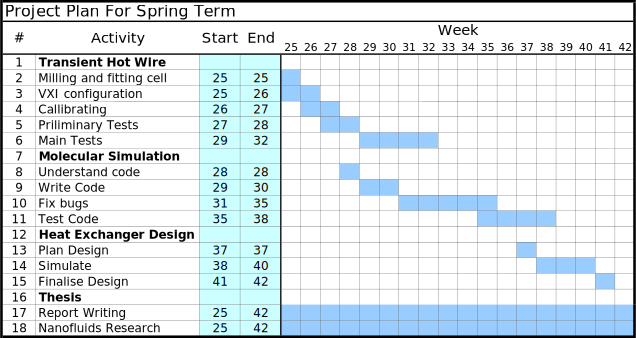
\includegraphics[clip,width=1\linewidth]{figures/Gchart.pdf}
  \caption{\label{fig:gchart} Expected spring term work flow.}
\end{figure}


\unchapter{Risk Assessment}
\includepdf[pages=1, angle=90, scale=0.95, pagecommand={\thispagestyle{plain}}]{RiskAssessment.pdf}
\includepdf[pages=2, angle=270, scale=0.95, pagecommand={\thispagestyle{plain}}]{RiskAssessment.pdf}
\printbibliography[heading=thesisChapterBib]

\includepdf[pages=1, scale=1, pagecommand={\thispagestyle{plain}}]{plag.pdf}
\end{document}
